%**************************************%
%* Generated from MathBook XML source *%
%*    on 2016-07-14T06:14:47-04:00    *%
%*                                    *%
%*   http://mathbook.pugetsound.edu   *%
%*                                    *%
%**************************************%
\documentclass[10pt,]{book}
%% Load geometry package to allow page margin adjustments
\usepackage{geometry}
\geometry{letterpaper,total={5.0in,9.0in}}
%% Custom Preamble Entries, early (use latex.preamble.early)
%% Inline math delimiters, \(, \), need to be robust
%% 2016-01-31:  latexrelease.sty  supersedes  fixltx2e.sty
%% If  latexrelease.sty  exists, bugfix is in kernel
%% If not, bugfix is in  fixltx2e.sty
%% See:  https://tug.org/TUGboat/tb36-3/tb114ltnews22.pdf
%% and read "Fewer fragile commands" in distribution's  latexchanges.pdf
\IfFileExists{latexrelease.sty}{}{\usepackage{fixltx2e}}
%% Page Layout Adjustments (latex.geometry)
%% This LaTeX file may be compiled with pdflatex or xelatex
%% The following provides engine-specific capabilities
%% Generally, xelatex will do better languages other than US English
%% You can pick from the conditional if you will only ever use one engine
\usepackage{ifthen}
\usepackage{ifxetex}
\ifthenelse{\boolean{xetex}}{%
%% begin: xelatex-specific configuration
%% fontspec package will make Latin Modern (lmodern) the default font
\usepackage{xltxtra}
\usepackage{fontspec}
%% end: xelatex-specific configuration
}{%
%% begin: pdflatex-specific configuration
%% translate common Unicode to their LaTeX equivalents
%% Also, fontenc with T1 makes CM-Super the default font
%% (\input{ix-utf8enc.dfu} from the "inputenx" package is possible addition (broken?)
\usepackage[T1]{fontenc}
\usepackage[utf8]{inputenc}
%% end: pdflatex-specific configuration
}
%% Monospace font: Inconsolata (zi4)
%% Sponsored by TUG: http://levien.com/type/myfonts/inconsolata.html
%% See package documentation for excellent instructions
%% One caveat, seem to need full file name to locate OTF files
%% Loads the "upquote" package as needed, so we don't have to
%% Upright quotes might come from the  textcomp  package, which we also use
%% We employ the shapely \ell to match Google Font version
%% pdflatex: "varqu" option produces best upright quotes
%% xelatex: add StylisticSet 1 for shapely \ell
%% xelatex: add StylisticSet 2 for plain zero
%% xelatex: we add StylisticSet 3 for upright quotes
%% 
\ifthenelse{\boolean{xetex}}{%
%% begin: xelatex-specific monospace font
\usepackage{zi4}
\setmonofont[BoldFont=Inconsolatazi4-Bold.otf,StylisticSet={1,3}]{Inconsolatazi4-Regular.otf}
%% end: xelatex-specific monospace font
}{%
%% begin: pdflatex-specific monospace font
\usepackage[varqu]{zi4}
%% end: pdflatex-specific monospace font
}
%% Symbols, align environment, bracket-matrix
\usepackage{amsmath}
\usepackage{amssymb}
%% allow more columns to a matrix
%% can make this even bigger by overriding with  latex.preamble.late  processing option
\setcounter{MaxMatrixCols}{30}
%% Semantic Macros
%% To preserve meaning in a LaTeX file
%% Only defined here if required in this document
%% Used for inline definitions of terms
\newcommand{\terminology}[1]{\textbf{#1}}
%% Subdivision Numbering, Chapters, Sections, Subsections, etc
%% Subdivision numbers may be turned off at some level ("depth")
%% A section *always* has depth 1, contrary to us counting from the document root
%% The latex default is 3.  If a larger number is present here, then
%% removing this command may make some cross-references ambiguous
%% The precursor variable $numbering-maxlevel is checked for consistency in the common XSL file
\setcounter{secnumdepth}{3}
%% Environments with amsthm package
%% Theorem-like environments in "plain" style, with or without proof
\usepackage{amsthm}
\theoremstyle{plain}
%% Numbering for Theorems, Conjectures, Examples, Figures, etc
%% Controlled by  numbering.theorems.level  processing parameter
%% Always need a theorem environment to set base numbering scheme
%% even if document has no theorems (but has other environments)
\newtheorem{theorem}{Theorem}[section]
%% Only variants actually used in document appear here
%% Style is like a theorem, and for statements without proofs
%% Numbering: all theorem-like numbered consecutively
%% i.e. Corollary 4.3 follows Theorem 4.2
%% Example-like environments, normal text
%% Numbering is in sync with theorems, etc
\theoremstyle{definition}
\newtheorem{example}[theorem]{Example}
%% Numbering for Projects (independent of others)
%% Controlled by  numbering.projects.level  processing parameter
%% Always need a project environment to set base numbering scheme
%% even if document has no projectss (but has other blocks)
\newtheorem{project}{Project}[section]
%% Project-like environments, normal text
\theoremstyle{definition}
\newtheorem{activity}[project]{Activity}
%% Miscellaneous environments, normal text
%% Numbering for inline exercises and lists is in sync with theorems, etc
\theoremstyle{definition}
\newtheorem{exercise}[theorem]{Exercise}
%% Localize LaTeX supplied names (possibly none)
\renewcommand*{\proofname}{Proof}
\renewcommand*{\appendixname}{Appendix}
\renewcommand*{\chaptername}{Chapter}
%% Figures, Tables, Listings, Floats
%% The [H]ere option of the float package fixes floats in-place,
%% in deference to web usage, where floats are totally irrelevant
%% We re/define the figure, table and listing environments, if used
%%   1) New mbxfigure and/or mbxtable environments are defined with float package
%%   2) Standard LaTeX environments redefined to use new environments
%%   3) Standard LaTeX environments redefined to step theorem counter
%%   4) Counter for new environments is set to the theorem counter before caption
%% You can remove all this figure/table setup, to restore standard LaTeX behavior
%% HOWEVER, numbering of figures/tables AND theorems/examples/remarks, etc
%% WILL ALL de-synchronize with the numbering in the HTML version
%% You can remove the [H] argument of the \newfloat command, to allow flotation and 
%% preserve numbering, BUT the numbering may then appear "out-of-order"
\usepackage{float}
\usepackage[bf]{caption} % http://tex.stackexchange.com/questions/95631/defining-a-new-type-of-floating-environment 
\usepackage{newfloat}
\usepackage{subcaption}
\captionsetup[subfigure]{labelformat=simple}
\captionsetup[subtable]{labelformat=simple}
\renewcommand\thesubfigure{(\alph{subfigure})}
\makeatletter
% we plan to use subtables within figure environments, so they need to reset accordingly
\@addtoreset{subtable}{figure}
\makeatother
% Side-by-side elements need careful treatement for aligning captions, see: 
% http://tex.stackexchange.com/questions/230335/vertically-aligning-minipages-subfigures-and-subtables-not-with-baseline 
\usepackage{stackengine,ifthen}
\newcounter{figstack}
\newcounter{figindex}
\newlength\fight
\newcommand\pushValignCaptionBottom[5][b]{%
\stepcounter{figstack}%
\expandafter\def\csname %
figalign\romannumeral\value{figstack}\endcsname{#1}%
\expandafter\def\csname %
figtype\romannumeral\value{figstack}\endcsname{#2}%
\expandafter\def\csname %
figwd\romannumeral\value{figstack}\endcsname{#3}%
\expandafter\def\csname %
figcontent\romannumeral\value{figstack}\endcsname{#4}%
\expandafter\def\csname %
figcap\romannumeral\value{figstack}\endcsname{#5}%
\setbox0=\hbox{%
\begin{#2}{#3}#4\end{#2}}%
\ifdim\dimexpr\ht0+\dp0\relax>\fight\global\setlength{\fight}{%
\dimexpr\ht0+\dp0\relax}\fi%
}
\newcommand\popValignCaptionBottom{%
\setcounter{figindex}{0}%
\hfill%
\whiledo{\value{figindex}<\value{figstack}}{%
\stepcounter{figindex}%
\def\tmp{\csname figwd\romannumeral\value{figindex}\endcsname}%
\begin{\csname figtype\romannumeral\value{figindex}\endcsname}[t]{\tmp}%
\centering%
\stackinset{c}{}%
{\csname figalign\romannumeral\value{figindex}\endcsname}{}%
{\csname figcontent\romannumeral\value{figindex}\endcsname}%
{\rule{0pt}{\fight}}\par%
\csname figcap\romannumeral\value{figindex}\endcsname%
\end{\csname figtype\romannumeral\value{figindex}\endcsname}%
\hfill%
}%
\setcounter{figstack}{0}%
\setlength{\fight}{0pt}%
\hfill%
}
% Figure environment setup so that it no longer floats
\SetupFloatingEnvironment{figure}{fileext=lof,placement={H},within=section,name=Figure}
% figures have the same number as theorems: http://tex.stackexchange.com/questions/16195/how-to-make-equations-figures-and-theorems-use-the-same-numbering-scheme 
\makeatletter
\let\c@figure\c@theorem
\makeatother
%% Footnote Numbering
%% We reset the footnote counter, as given by numbering.footnotes.level
\makeatletter\@addtoreset{footnote}{section}\makeatother
%% Raster graphics inclusion, wrapped figures in paragraphs
\usepackage{graphicx}
%% Colors for Sage boxes, author tools (red hilites), red/green edits
\usepackage[usenames,dvipsnames,svgnames,table]{xcolor}
%% Program listing support, for inline code, Sage code
\usepackage{listings}
%% We define the listings font style to be the default "ttfamily"
%% To fix hyphens/dashes rendered in PDF as fancy minus signs by listing
%% http://tex.stackexchange.com/questions/33185/listings-package-changes-hyphens-to-minus-signs
\makeatletter
\lst@CCPutMacro\lst@ProcessOther {"2D}{\lst@ttfamily{-{}}{-{}}}
\@empty\z@\@empty
\makeatother
%% End of generic listing adjustments
%% Inline code, typically from "c" element
%% Global, document-wide options apply to \lstinline
%% Search/replace \lstinline by \verb to remove this dependency
%% (redefining \lstinline with \verb is unlikely to work)
%% Also see "\renewcommand\UrlFont" below for matching font choice
\lstset{basicstyle=\small\ttfamily,breaklines=true,breakatwhitespace=true}
%% More flexible list management, esp. for references and exercises
%% But also for specifying labels (i.e. custom order) on nested lists
\usepackage{enumitem}
%% Lists of exercises in their own section, maximum depth 4
\newlist{exerciselist}{description}{4}
\setlist[exerciselist]{leftmargin=0pt,itemsep=1.0ex,topsep=1.0ex,partopsep=0pt,parsep=0pt}
%% Package for breakable boxes on WeBWorK problems from server LaTeX
\usepackage{mdframed}
%% WeBWorK problem style
\mdfdefinestyle{webwork-server}{framemethod=default, linewidth=2pt}
%% hyperref driver does not need to be specified
\usepackage{hyperref}
%% Hyperlinking active in PDFs, all links solid and blue
\hypersetup{colorlinks=true,linkcolor=blue,citecolor=blue,filecolor=blue,urlcolor=blue}
\hypersetup{pdftitle={Active Calculus - Single Variable}}
%% If you manually remove hyperref, leave in this next command
\providecommand\phantomsection{}
%% If tikz has been loaded, replace ampersand with \amp macro
%% extpfeil package for certain extensible arrows,
%% as also provided by MathJax extension of the same name
%% NB: this package loads mtools, which loads calc, which redefines
%%     \setlength, so it can be removed if it seems to be in the 
%%     way and your math does not use:
%%     
%%     \xtwoheadrightarrow, \xtwoheadleftarrow, \xmapsto, \xlongequal, \xtofrom
%%     
%%     we have had to be extra careful with variable thickness
%%     lines in tables, and so also load this package late
\usepackage{extpfeil}
%% Custom Preamble Entries, late (use latex.preamble.late)
%% Begin: Author-provided macros
%% (From  docinfo/macros  element)
%% Plus three from MBX for XML characters

\newcommand{\lt}{ < }
\newcommand{\gt}{ > }
\newcommand{\amp}{ & }
%% End: Author-provided macros
%% Title page information for book
\title{Active Calculus - Single Variable\\
{\large This is Only a Test}}
\author{}
\date{}
\begin{document}
\typeout{************************************************}
\typeout{Chapter 1 My first chapter}
\typeout{************************************************}
\chapter[My first chapter]{My first chapter}\label{ch-1}
\typeout{************************************************}
\typeout{Introduction  }
\typeout{************************************************}
In this chapter of the text, we investigate several different standard things that we need to do in writing an MBX text, including how to include graphics, use knowls, and include exercises.%
\typeout{************************************************}
\typeout{Section 1.1 Graphics and other Basics}
\typeout{************************************************}
\section[Graphics and other Basics]{Graphics and other Basics}\label{ch-1-velocity}
\typeout{************************************************}
\typeout{Introduction  }
\typeout{************************************************}
 In this section of the text, we are trying to understand some basic MBX features, including %
\leavevmode%
\begin{itemize}[label=\textbullet]
\item{}how to make an unordered list%
\item{}how to effectively use Sublime%
\item{}how to use math mode to write things like \(f'(x) = \lim_{h \to 0} \frac{f(x+h) - f(x)}{h}\)%
\item{}how to include graphics and resize them%
\end{itemize}
\typeout{************************************************}
\typeout{Subsection 1.1.1 Including Graphics}
\typeout{************************************************}
\subsection[Including Graphics]{Including Graphics}\label{subsection-1}
To include a plot, we need to use the PDF to SVG utility (pdf2svg), and even before that need to use epstopdf.  I need to learn more about how all this works with HomeBrew from the Terminal line.  Should we use the filename (which is sort of a title) as the label, too? %
\leavevmode%
\begin{figure}
\centering
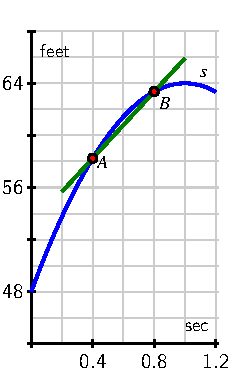
\includegraphics[width=0.50\textwidth,]{images/act-sec-soln.pdf}\caption{This is the caption for the figure. \label{test_figure_1}}
\end{figure}
\par
I need to think carefully about how subsections will be structured.%
\par
How will we address the size of graphics?%
\leavevmode%
\begin{figure}
\centering
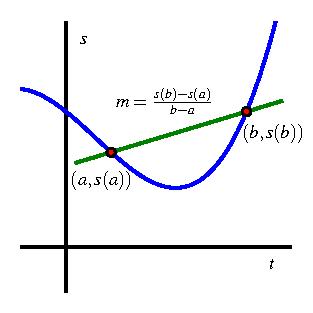
\includegraphics[width=0.50\textwidth,]{images/der-vel-summary.pdf}\caption{Is this figure smaller? \label{test_figure_2}}
\end{figure}
\typeout{************************************************}
\typeout{Subsection 1.1.2 This is the title of my second subsection}
\typeout{************************************************}
\subsection[This is the title of my second subsection]{This is the title of my second subsection}\label{subsection-2}
This is text in the second subsection, and below is an example of a side-by-side figure.%
\leavevmode%
\begin{figure}
\centering
\pushValignCaptionBottom[b]{subfigure}{.50\textwidth}{%
\centering% horizontal alignment 
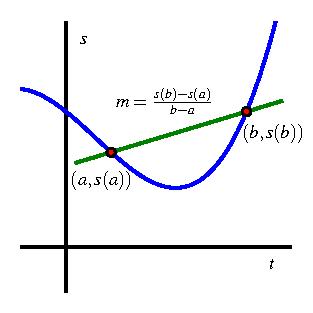
\includegraphics[width=\textwidth,]{images/der-vel-summary.pdf}}% end body 
{\caption{\label{fig-sidebyside-subfigure}}
}% caption 
\pushValignCaptionBottom[b]{subfigure}{.50\textwidth}{%
\centering% horizontal alignment 
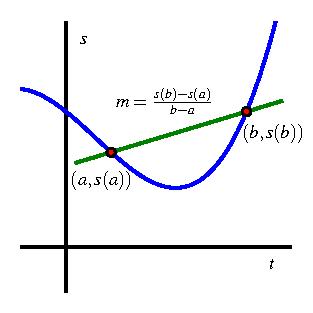
\includegraphics[width=\textwidth,]{images/der-vel-summary.pdf}}% end body 
{\caption{\label{figure-4}}
}% caption 
\popValignCaptionBottom
\caption{Side-by-side Figure, with subfigure children.\label{fig-sidebyside-global}}
\end{figure}
\typeout{************************************************}
\typeout{Section 1.2 Using Knowls}
\typeout{************************************************}
\section[Using Knowls]{Using Knowls}\label{ch-1-limit}
\typeout{************************************************}
\typeout{Introduction  }
\typeout{************************************************}
 In this section of the text, we will explore the use of \terminology{knowls}. %
\typeout{************************************************}
\typeout{Subsection 1.2.1 Things that are automatically knowl-ized}
\typeout{************************************************}
\subsection[Things that are automatically knowl-ized]{Things that are automatically knowl-ized}\label{subsection-3}
Footnotes are even better as knowls.\footnote{Because they appear adjacent to the footnote in the text when you click on them.\label{fn-1}}%
\par
If we do a theorem that has a proof, the proof is automatically in a knowl.  The theorem structure in MBX also has several key levels/components:  theorem, title, index, statement, proof.%
\begin{theorem}[My Theorem]\label{theorem-MyTheorem}
\index{}If a triangle has sides of length \(a\), \(b\), and \(c\), and \(a^2 + b^2 = c^2\), then the triangle is a right triangle.%
\end{theorem}
\begin{proof}\hypertarget{proof-1}{}
Here is my insightful argument.%
\end{proof}
\par
Examples are also automatically put into knowls.%
\begin{example}[]\label{example-ch-1-MyExample}
 Here is an example application of Theorem \hyperref[theorem-MyTheorem]{\ref{theorem-MyTheorem}}.  Suppose that we have a triangle whose sides are of length 5, 12, 13.  Then, since \(5^2 + 12^2 = 25 + 144 = 169 = 13^2\), it follows that the triangle must be a right triangle.%
\end{example}
\typeout{************************************************}
\typeout{Subsection 1.2.2 How do exercises work?}
\typeout{************************************************}
\subsection[How do exercises work?]{How do exercises work?}\label{subsection-4}
Exercises seem to be set up so that they appear as their own section.  Can we put them within a subsection?  Is this one of the things Rob is working on?%
\typeout{************************************************}
\typeout{Section 1.3 Using Activities}
\typeout{************************************************}
\section[Using Activities]{Using Activities}\label{ch-1-activities}
\typeout{************************************************}
\typeout{Introduction  }
\typeout{************************************************}
 In this section of the text, we will explore the use of \terminology{activities} and think about issues like how we deal with there not yet being an "activities" environment in MBX and where to put solutions.  Really, how are activities different from exercises? %
\typeout{************************************************}
\typeout{Subsection 1.3.1 How does the exercise environment work?}
\typeout{************************************************}
\subsection[How does the exercise environment work?]{How does the exercise environment work?}\label{subsection-5}
Exercises seem to be set up so that they appear as their own section.  Can we put them within a subsection?  Is this one of the things Rob is working on?%
\par
Exercises also, when included in the "exercises" environment, appear with their full statement included.  When included as a single "exercise", such as the one following, appear as knowls.%
\begin{exercise}[Essay Question: Compare and Contrast]\label{exercise-essay}
Write a short paragraph that compares and contrasts the definite and indefinite integral. This is an exercise that sits in the midst of the narrative, so is formatted more like an example or a remark.  It can have a hint and a solution, but this one does not.  It can have a title, which this one does.%
\par\smallskip
\noindent\textbf{Hint.}\hypertarget{hint-1}{}\quad
Start writing!%
\end{exercise}
\par
I wonder if all activities could just be called exercises.  Or if Rob is open to having an environment identical to "exercise" that's called "activity".%
\par
Here is an activity directly from \emph{Active Calculus}.%
\begin{exercise}[Car on a straight road]\label{act-car-concavity}

				The position of a car driving along a straight road at time \(t\) in minutes is given by the function \(y = s(t)\) that is pictured in \hyperref[act-car-graph]{Figure~\ref{act-car-graph}}. The car's position function has units measured in thousands of feet. Remember that you worked with this function and sketched graphs of \(y = v(t) = s'(t)\) and \(y = v'(t)\) in a previous activity . %
\leavevmode%
\begin{figure}
\centering
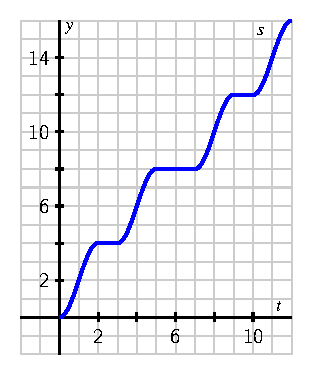
\includegraphics[width=0.50\textwidth,]{images/act-car-graph.pdf}\caption{The graph of \(y = s(t)\), the position of the car (measured in thousands of feet from its starting location) at time \(t\) in minutes.\label{act-car-graph}}
\end{figure}
\leavevmode%
\begin{enumerate}
\item\hypertarget{li-5}{}On what intervals is the position function \(y = s(t)\) increasing? decreasing?  Why?\item\hypertarget{li-6}{}On which intervals is the velocity function \(y = v(t) = s'(t)\) increasing? decreasing? neither?  Why?\item\hypertarget{li-7}{}\emph{Acceleration} is defined to be the instantaneous rate of change of velocity, as the acceleration of an object measures the rate at which the velocity of the object is changing.  Say that the car's acceleration function is named \(a(t)\).  How is \(a(t)\) computed from \(v(t)\)?  How is \(a(t)\) computed from \(s(t)\)?  Explain.\item\hypertarget{li-8}{}What can you say about \(s''\) whenever \(s'\) is increasing?  Why?\item\hypertarget{li-9}{}Using only the words \emph{increasing}, \emph{decreasing}, \emph{constant}, \emph{concave up}, \emph{concave down}, and \emph{linear}, complete the following sentences.  For the position function \(s\) with velocity \(v\) and acceleration \(a\),
					\begin{itemize}[label=\textbullet]
\item{}on an interval where \(v\) is positive, \(s\) is .\item{}on an interval where \(v\) is negative, \(s\) is .\item{}on an interval where \(v\) is zero, \(s\) is .\item{}on an interval where \(a\) is positive, \(v\) is .\item{}on an interval where \(a\) is negative, \(v\) is .\item{}on an interval where \(a\) is zero, \(v\) is .\item{}on an interval where \(a\) is positive, \(s\) is .\item{}on an interval where \(a\) is negative, \(s\) is .\item{}on an interval where \(a\) is zero, \(s\) is .\end{itemize}
\end{enumerate}
\par\smallskip
\noindent\textbf{Hint.}\hypertarget{hint-2}{}\quad
Exercises (and presumably activities) can have hints.\par\smallskip
\noindent\textbf{Solution.}\hypertarget{solution-1}{}\quad
And some exercises/activities will have solutions\end{exercise}
\par
I need to understand how to make the "solution" and "answer" options not appear with the exercise/activity, and yet to have these available at the end.%
\typeout{************************************************}
\typeout{Subsection 1.3.2 How does the new "Activity" environment work?}
\typeout{************************************************}
\subsection[How does the new "Activity" environment work?]{How does the new "Activity" environment work?}\label{subsection-6}
Rob instantiated this feature at my request in mid-June 2016.%
\begin{activity}[An Example of an Activity]\label{sample-activity}
An \lstinline?activity? behaves identically to \lstinline?example?s; they may have an independent numbering scheme.  There does not appear to be a "solution" feature; need to learn how to keep these separate.%

                        	Here is a hint to the activity
                        
                        	If I want to provide an answer to an activity, I can.
                        \par\medskip\noindent%
\textbf{Solution.}\quad  Is there a solution?  If yes, how do I make it appear elsewhere? %
\end{activity}
\typeout{************************************************}
\typeout{Exercises 1.4 Exercises}
\typeout{************************************************}
\section[Exercises]{Exercises}\label{exercises-sets}
\begin{exerciselist}
\item[1.]\hypertarget{exercises-sets-trial}{}
			This is the statement of my first exercise.
		\par\smallskip
\par\smallskip
\noindent\textbf{Hint.}\hypertarget{hint-4}{}\quad

			And this is a hint.
		\item[2.]\hypertarget{exercises-sets-with-solution}{}
			Suppose that an object moving along an axis has instantaneous velocity \(v(t) = 2t-3\) and its position at time \(t=1\) is \(s(1) = -1\).  What is the position of the object at \(t = 5\)?
		\par\smallskip
\par\smallskip
\noindent\textbf{Hint.}\hypertarget{hint-5}{}\quad
 Don't forget that the velocity function is the derivative of position. \par\smallskip
\noindent\textbf{Answer.}\hypertarget{answer-3}{}\quad
\(s(5) = 11\)\par\smallskip
\noindent\textbf{Solution.}\hypertarget{solution-3}{}\quad
Since \(v(t) = 2t-3\), it follows that \(s(t) = t^2 - 3t + C\).  Moreover, because \(s(1)=-1\), we see that \(-1 = 1^2 - 3 \cdot 1 + C\), co \(C = 1\).  Thus, \(s(t) = t^2 - 3t + 1\), and \(s(5) = 11\). \item[3.]\hypertarget{exercises-sets-with-answer}{}
			Here's one more new exercise.
		\par\smallskip
\par\smallskip
\noindent\textbf{Answer.}\hypertarget{answer-4}{}\quad
7\item[4.]\hypertarget{exercises-sets-test}{}
			Here's a second exercise, but without a hint.
		\par\smallskip
\item[5.]\hypertarget{exercises-sets-with-webwork}{}\typeout{************************************************}
\typeout{Introduction  }
\typeout{************************************************}
 Next I'm going to try to add a WeBWorK exercise via PCC's server: %
\mbox{}\\ % hack to move box after heading
\begin{mdframed}
{}\par\vspace*{2ex}%
{\tiny\ttfamily\noindent
Library/Rochester/setIntegrals4FTC/S05.03.FundThmCalc.PTP01.pg\\Seed: \hfill}\end{mdframed}
\item[6.]\hypertarget{exercises-sets-with-webwork-2}{}\typeout{************************************************}
\typeout{Introduction  }
\typeout{************************************************}
Here's a second WeBWorK exercise, borrowing from a Math 201 def file.%
\mbox{}\\ % hack to move box after heading
\begin{mdframed}
{}\par\vspace*{2ex}%
{\tiny\ttfamily\noindent
Library/Michigan/Chap3Sec4/Q47.pg\\Seed: \hfill}\end{mdframed}
\end{exerciselist}
%
%% A lineskip in table of contents as transition to appendices, backmatter
\addtocontents{toc}{\vspace{\normalbaselineskip}}
%
%
\appendix
%
\typeout{************************************************}
\typeout{Appendix A Hints and Solutions to Selected Exercises}
\typeout{************************************************}
\chapter[Hints and Solutions to Selected Exercises]{Hints and Solutions to Selected Exercises}\label{appendix-1}
\section*{1.4 Exercises}
\noindent\textbf{1.}\quad{}
			This is the statement of my first exercise.
		\par\smallskip

			And this is a hint.
		\par\smallskip
\noindent\textbf{2.}\quad{}
			Suppose that an object moving along an axis has instantaneous velocity \(v(t) = 2t-3\) and its position at time \(t=1\) is \(s(1) = -1\).  What is the position of the object at \(t = 5\)?
		\par\smallskip
 Don't forget that the velocity function is the derivative of position. \par\smallskip
\(s(5) = 11\)\par\smallskip
Since \(v(t) = 2t-3\), it follows that \(s(t) = t^2 - 3t + C\).  Moreover, because \(s(1)=-1\), we see that \(-1 = 1^2 - 3 \cdot 1 + C\), co \(C = 1\).  Thus, \(s(t) = t^2 - 3t + 1\), and \(s(5) = 11\). \par\smallskip
\noindent\textbf{3.}\quad{}
			Here's one more new exercise.
		\par\smallskip
7\par\smallskip
%
\backmatter
%
\end{document}